\subsection{}
\begin{definition}
    \emph{Consumer Surplus} is the difference in the maximum the consumer is willing to pay 
    and what is actually paid. Consumer surplus increases for three reasons.
    \begin{enumerate}
        \item the more inelastic the demand curve is.
        \item the lower the price is.
        \item if the demand curve shifts.
    \end{enumerate}
\end{definition}
The maximum willingness to pay is reflected in the demand curve.\\
The consumer surplus is the area under the demand curve and above the price.
\begin{figure}[H]
    \centering
    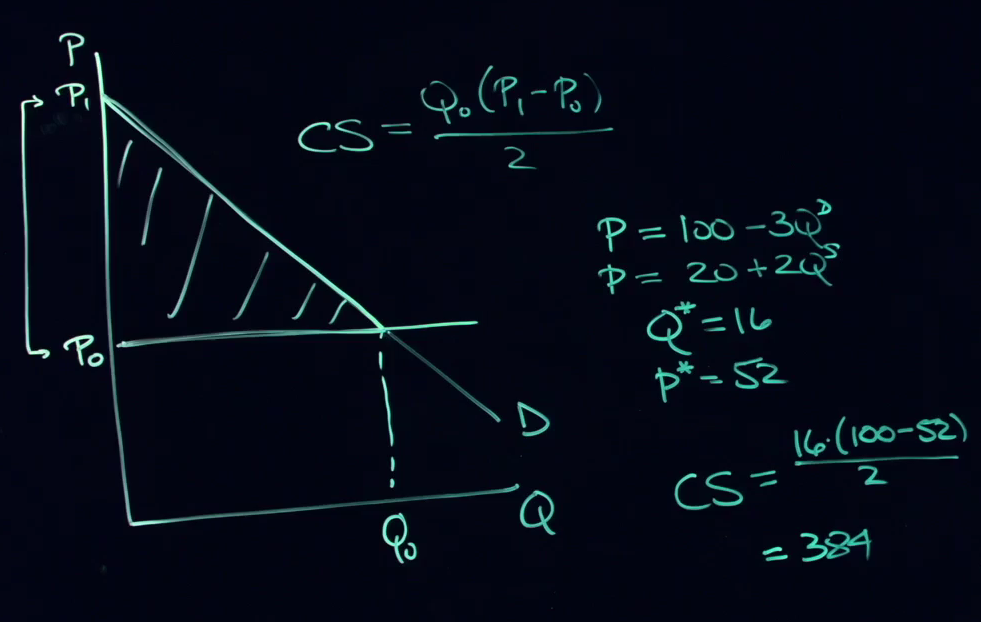
\includegraphics[width=0.5\textwidth]{Chapter6/ConsumerSurplus.png}
    \caption{Consumer Surplus}
    \label{fig:Consumer_Surplus}
\end{figure}
\begin{definition}
    \emph{Paradox of Value}. Think about water being essential for life, but reasonably cheap. Diamonds are not essential, but are expensive.
    The paradox was resolved because water is abundant and diamonds are scarce. We are willing to pay much more for water.
\end{definition}
\begin{figure}[H]
    \centering
    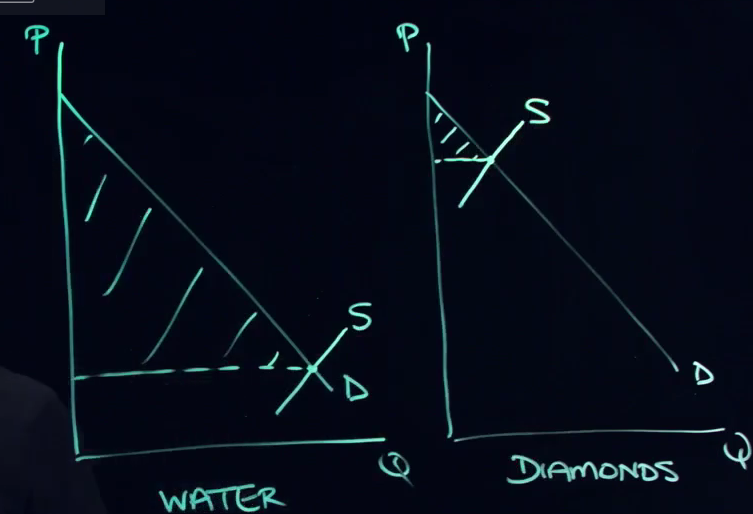
\includegraphics[width=0.5\textwidth]{Chapter6/ParadoxofValue.png}
    \caption{Paradox of Value}
    \label{fig:Paradox_of_Value}
\end{figure}